\section{Auswertung}
\label{sec:Auswertung}


\begin{table}[!htp]
  \begin{minipage}{0.5\linewidth}
    \centering
    \begin{tabular}{
      S[table-format=2.2]
      S[table-format=1.2]
    }
      \toprule
      {$t_{hoch}\left[\unit{\s}\right]$} & {$t_{runter}\left[\unit{\s}\right]$}\\
      \midrule
      12.85 & 12.97\\
      12.97 & 13.10\\
      13.00 & 12.85\\
      13.00 & 12.94\\
      13.00 & 13.13\\
      13.07 & 13.00\\
      13.05 & 13.03\\
      13.13 & 13.00\\
      12.97 & 13.12\\
      13.03 & 13.12\\
      \bottomrule
    \end{tabular}
    \vspace{5pt}
    \caption{Fallzeiten der kleinen\\ Kugel bei Raumtemperatur}
    \label{table:kk}
  \end{minipage}
  \begin{minipage}{0.5\linewidth}
    \centering
    \begin{tabular}{|c|c|}
      \hline
      {$t_{hoch}\left[\unit{\s}\right]$} & {$t_{runter}\left[\unit{\s}\right]$}\\
      \hline    
      52.53 & 52.78\\
      53.19 & 52.38\\
      53.79 & 52.97\\
      53.69 & 53.16\\
      53.53 & 53.19\\
      \hline
    \end{tabular}
    \vspace{5pt}
    \caption{Fallzeiten der großen\\ Kugel bei Raumtemperatur}
    \label{table:gk}
  \end{minipage}
\end{table}

Die mittlere Fallzeit kann mit \ref{eqn:6} berechnet werden.\\
Gemittelte Fallzeiten kleine Kugel: \qquad \qquad \qquad \qquad Große Kugel:
\begin{align}
  \bar{t}_{\text{hoch}} &= 13.007\,\unit{\second}  \quad &\bar{t}_{\text{hoch}} &= 53.346\,\unit{\second}\\
  \bar{t}_{\text{runter}} &= 13.026\,\unit{\second}  \quad &\bar{t}_{\text{hoch}} &= 52.896\,\unit{\second}\\
  \bar{t}_{\text{gesamt}} &= 13.0165\,\unit{\second}  \quad &\bar{t}_{\text{gesamt}} &= 53.121\,\unit{\second}
\end{align}

Mit den Werten der Tabelle \ref{table:gk} rechnen wir mit Formel \ref{eqn:K}
die Aparatekonstante $K$ aus. Dafür muss zuerst $η$ mit den Werten aus Tabelle \ref{table:kk} berechnen.\\
Der Fehler wird mit \ref{eqn:8} berechnet. Der Wert für $K_{Kl}$ ist in der Aufgabenstellung gegeben.\\
\begin{equation}
  η = 0.07640\,\mathrm{mPacm^3g^{-1}} \cdot 
\end{equation}



\begin{table}[!htp]
  \centering
  \begin{tabular}{|c|c|c|}
    \hline
    $T [\unit{\degreeCelsius}]$ & $t_{runter} [\unit{\second}]$ & $t_{hoch} [\unit{\second}]$\\
    \hline \hline
    27.5 & 47.5 & 46\\
    27.5 & 45 & 43.97\\
    29 & 43.47 & 42.97\\
    29 & 44.13 & 42.81\\
    30.5 & 42.19 & 41.59\\
    30.5 & 42.4 & 41.34\\
    32 & 41.69 & 41.12\\
    32 & 41.91 & 40.66\\
    39.5 & 36.03 & 35.15\\
    39.5 & 35.41 & 35.53\\
    47 & 32.18 & 31.03\\
    47 & 31.66 & 30.79\\
    50 & 30.38 & 29.97\\
    50 & 29.91 & 29.34\\
    52 & 28.63 & 28.22\\
    52 & 28.91 & 28.22\\
    56 & 27.03 & 26.53\\
    56 & 26.88 & 26.85\\
  \end{tabular}
  \label{tabellegkt}
  \caption{Fallzeiten der großen Kugel bei steigender Temperatur}
\end{table}

%\begin{figure}
%  \centering
%  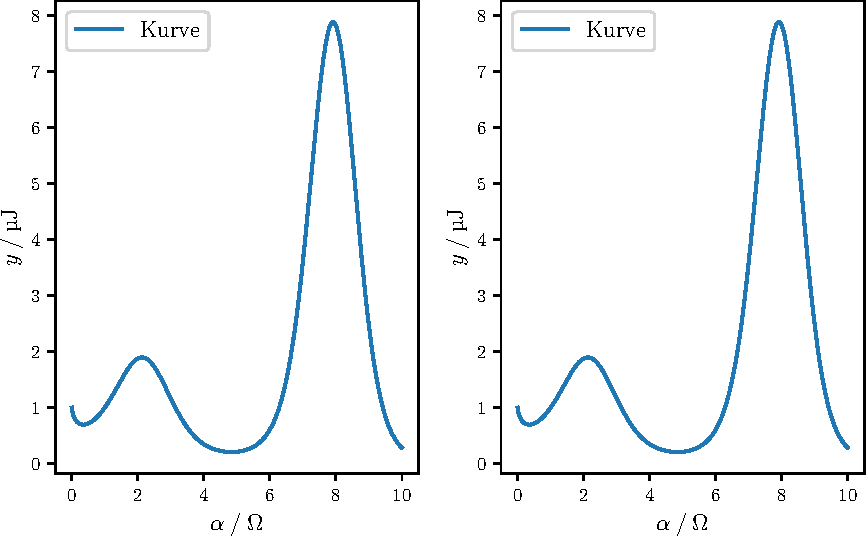
\includegraphics{plot.pdf}
%  \caption{Plot.}
%  \label{fig:plot}
%\end{figure}

%Siehe \autoref{fig:plot}!